\documentclass[fleqn]{article}
\oddsidemargin 0.0in
\textwidth 6.0in
\thispagestyle{empty}
\usepackage{import}
\usepackage{amsmath}
\usepackage{graphicx}
\usepackage{flexisym}
\usepackage{calligra}
\usepackage{amssymb}
\usepackage{bigints} 
\usepackage[english]{babel}
\usepackage[utf8x]{inputenc}
\usepackage{float}
\usepackage[colorinlistoftodos]{todonotes}


\DeclareMathAlphabet{\mathcalligra}{T1}{calligra}{m}{n}
\DeclareFontShape{T1}{calligra}{m}{n}{<->s*[2.2]callig15}{}
\newcommand{\scriptr}{\mathcalligra{r}\,}
\newcommand{\boldscriptr}{\pmb{\mathcalligra{r}}\,}

\definecolor{hwColor}{HTML}{442020}

\begin{document}

  \begin{titlepage}

    \newcommand{\HRule}{\rule{\linewidth}{0.5mm}}

    \center

    \begin{center}
      
\includegraphics[height=11cm, width=11cm]{asu.png}
    \end{center}

    \vline

    \textsc{\LARGE Statistical/Thermal Physics}\\[1.5cm]

    \HRule \\[0.5cm]
    { \huge \bfseries Homework 2}\\[0.4cm] 
    \HRule \\[1.0cm]

    \textbf{Behnam Amiri}

    \bigbreak

    \textbf{Prof: Michael Treacy}

    \bigbreak

    \textbf{{\large \today}\\[2cm]}

    \vfill

  \end{titlepage}

  \begin{enumerate}
    \item \textbf{1.29} A cup containing $200 ~ g$ of water is sitting on your dining room table. After carefully measuring its 
    temperature to be $20^{\circ} ~ C$ you leave the room. Returning ten minutes later, you measure its temperature again 
    and find that it is now $25^{\circ} ~ C$. What you can conclude about the amount of heat added to the water?

    [Hint: This is a trick question.]

      \textcolor{hwColor}{
        \\
        From page 28 of the textbook we have:
        \\
        \\
        $
          \begin{cases}
            C=\dfrac{Q}{\Delta T}
            \\
            \\
            c \equiv \dfrac{C}{m}
          \end{cases} \Longrightarrow \boxed{Q=mc \Delta T} ~~~~ \checkmark
          \\
          \\
          \\
          \begin{cases}
            m=\bigg( \dfrac{200}{1000} ~ kg \bigg)
            \\
            \\
            m=4184 ~ J/kg.K ~~~ \text{Heat capacity of water}
            \\
            \\
            \Delta T= \bigg( 298.15 - 293.15 \bigg) ~ K ~~~ \text{Converted to Kelvin}
          \end{cases}
          \\
          \\
          \\
          Q=mc \Delta T=\bigg( \dfrac{200}{1000} ~ kg \bigg) \bigg( 4184 ~ J/kg.K \bigg) \bigg( 298.15 - 293.15 ~ K\bigg)
          \\
          \\
          \\
          \therefore ~~~ \boxed{
            Q=4184 ~ J
          } ~~~~ \checkmark
          \\
          \\
        $
        We have a $5^{\circ}$ increase in the temperature of the cup containing water which means there should have been
        $\approx 4184 ~ J$ energy entered the cup whether by a heater next to the cup or maybe the cup was placed in 
        the direct sun light. I can \emph{not} tell or conclude how the energy was added to the water maybe as heat or what 
        the source of the enrgy was.
        \\ 
      }

    \pagebreak

    \item \textbf{1.31} Imagine some helium in a cylinder with an intial volume of $1 ~ liter$ and an initial
    pressure of $1 ~ atm$. Somehow the helium is made to expand to a final volume of 3 liters, in such a way 
    that its pressure rises in direct proportion to its volume.
    \begin{enumerate}
      \item Sketch a graph of pressure vs.volume for this process.

      \begin{center}
        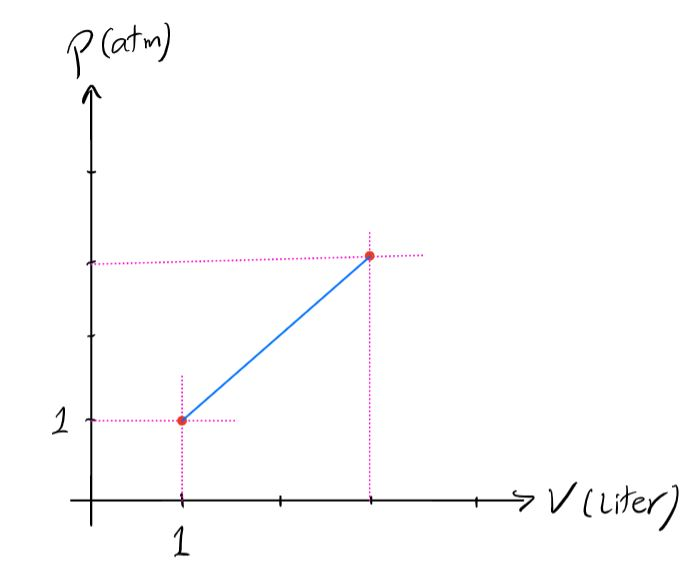
\includegraphics[height=8cm, width=11cm]{2.JPG}
      \end{center}

      \item Calculate the work done on the gas during this process, assuming that there are no "other"
      types of work being done.

        \textcolor{hwColor}{
          \\
          The area under the graph can be split into two standard shapes; A triangle and rectangle. Based on the assumtion 
          that there are no other types of work being done, and with the help of equation (1.28) we have the following result. 
          \\
          \\
          $
            W=-P ~ \Delta V=-\bigg( 2 ~ liters \times 1 ~ atm\bigg)+ \bigg( \dfrac{2 ~ liters \times 2 atm}{2} \bigg)
            \\
            \\
            =-\bigg( 0.002 ~ m^3 \times 101325 ~ N/m^2 \bigg)+ \bigg( \dfrac{ 0.002 ~ m^3 \times 202650 ~ N/m^2 }{2} \bigg)
            \\
            \\
            \\
            \therefore ~~~ \boxed{
              W=-405.3 ~ J
            } ~~~~ \checkmark
            \\
            \\
          $ 
        }

      \item Calculate the change in the helium's energy content during this process.

        \textcolor{hwColor}{
          \\
          From quiz one I learned that Helium atoms have three degrees of freedom, therefore their thermal energy can be calculated 
          with the following formula:
          \\
          \\
          $
            U=\dfrac{3}{2} ~ N K_B ~ T=\dfrac{3}{2} PV 
            \\
            \\
            \Delta U=\dfrac{3}{2} \left[U_f-U_i\right]
            =\dfrac{3}{2} \left[P_f V_f-P_f V_f\right]
            =\dfrac{3}{2} \left[
              \bigg( 3 ~ atm \times 3 ~ liters \bigg)
              -
              \bigg( 1 ~ atm \times 1 ~ liters \bigg)
            \right]
            \\
            \\
            \\
            =\dfrac{3}{2} \left[
              \bigg( 303975 ~ N/m^2 \times 0.003 ~ m^3 \bigg)
              -
              \bigg( 101325 ~ N/m^2 \times 0.001 ~ m^3 \bigg)
            \right]
            \\
            \\
            \\
            \therefore ~~~ \boxed{
              \Delta U \approx 1215.9 ~ J
            } ~~~~ \checkmark
            \\
            \\
          $
        }

      \item Calculate the amount of heat added to or removed from the helium during this process.

        \textcolor{hwColor}{
          \\
          $
            Q=\Delta U-W=1215.9-\bigg(-405.3 \bigg)
            \\
            \\
            \\
            \therefore ~~~ \boxed{
              Q=1621.2 ~ J
            } ~~~~ \checkmark
            \\
            \\
          $
        }

      \item Describe what you might do to cause the pressure to rise as the helium expands.

        \textcolor{hwColor}{
          \\
          One way can be to increase the temperature of the gas by holding fire under the cylinder containing Helium. With 
          the increase in the heat, the pressure rises too.
        }

    \end{enumerate}

    \pagebreak

    \item \textbf{1.33} an ideal gas is made to undergo the cyclic process shown in Figure 1.10(a). For
    each of the steps A, B, and C, determine whether each of the following is positive, negative , or zero: 
    (a) the work done on the gas; (b) the change in the energy content of the gas; (c) the heat added to the gas. 
    Then determine the sign of each of these three quantities for the whole cycle. What does this process accomplish?

    \begin{center}
      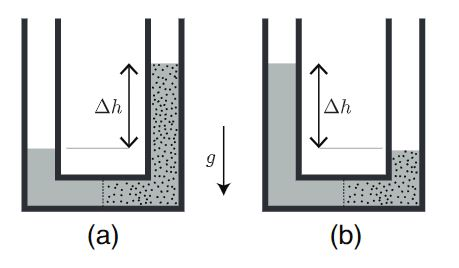
\includegraphics[height=7cm, width=16cm]{1.JPG}
    \end{center}

      % \textcolor{hwColor}{
      %   \\
      % }

    \item \textbf{1.34} An ideal gas diatomic gas, in a cylinder with a movable piston, undergoes the rectangular cyclic process
    shown in Figure 1.10(b). Assume that the temperature is always such that rotational degress of freedom are active, but vibrational
    modes are "frozen out". Also assume that the only type of work done on the gas is quasistatic compression-expansion work.
    \begin{enumerate}
      \item For each of the four steps A through D, compute the work done on the gas, the heat added to the gas, and the change in the energy
      content of the gas. Express all answers in terms of $P_1, P_2, V_1$, and $V_2$. (Hint: Compute $\Delta U$ before Q, using
      the ideal gas law and the equipartition theorem.)

        % \textcolor{hwColor}{
        %   \\
        % }

      \item Describe in words what is physically being done during each of the four steps; for example, during step A, heat is added to the 
      gas (from an external flame or something) while the piston is held fixed.
    
        % \textcolor{hwColor}{
        %   \\
        % }

      \item Compute the net work done on the gas, the net heat added to the gas, and the net change in the energy of the gas during the entire
      cycle. Are the results as you expected? Explain briefly.

        % \textcolor{hwColor}{
        %   \\
        % }

    \end{enumerate}


    \item \textbf{1.35} Derive equation $1.40$ from equation $1.39$.
  
        % \textcolor{hwColor}{
        %   \\
        % }

    \item \textbf{1.36} In the course of pumping up a bicycle tire, a liter of air at atmospheric pressure is compressed adiabatically 
    to a pressure of $7 ~ atm$. (Air is mostly diatomic nitrogen and oxygen.)
    \begin{enumerate}
      \item What is the final volume of this air after compression?

        % \textcolor{hwColor}{
        %   \\
        % }

      \item How much work is done in compressing the air?

        % \textcolor{hwColor}{
        %   \\
        % }
      
      \item If the temperature of the air is initially $300 ~ K$, what is the temperature after compression?

        % \textcolor{hwColor}{
        %   \\
        % }

    \end{enumerate}


    \item \textbf{1.42} The specific heat capacity of Albertson's \emph{Rotini Tricolore} is approximately $1.8 ~ J/g.^{\circ}C$. Suppose 
    you toss 340 g of this pasta (at $25^{\circ}C$) into 1.5 liters of boling water. What effect does this have on the temperature of the
    water (before there is time for the stove to provide more heat)?

        % \textcolor{hwColor}{
        %   \\
        % }

  \end{enumerate}

\end{document}
